\subsection{概述}
\label{subsec:arch}

\begin{figure}[t]
\centering
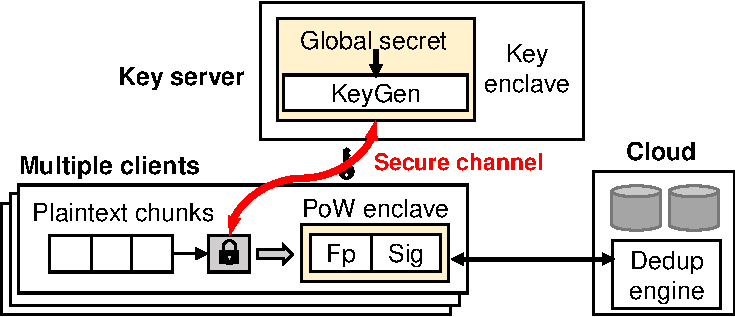
\includegraphics[width=3.3in]{pic/sgxdedup/overview.pdf}
\vspace{-3pt}
\caption{\sysname 架构概述:密钥服务器和每个客户端分别部署了一个密钥安全区和一个 PoW 安全区。}
\label{fig:overview}
\vspace{-3pt}
\end{figure}

\noindent{\bf 架构.} 图~\ref{fig:overview} 展示了 \sysname 的架构,其中引入了两个 enclave:{\em key enclave} 和 {\em PoW enclave}。 \sysname 在密钥服务器中部署一个密钥安全区,以管理和保护服务器辅助 MLE 的全局机密,使其免受受损密钥服务器的侵害。要执行 MLE 密钥生成,密钥安全区和客户端都首先基于共享 {\em 盲密钥} 建立一个安全通道(有关如何形成盲密钥的详细信息,请参阅 \S\ref{subsec:key-management}) .然后客户端通过安全通道提交明文块的指纹。密钥安全区计算 MLE 密钥作为全局秘密和指纹的加密哈希。它通过安全通道返回 MLE 密钥。

密钥安全区有利于性能和安全性。它避免了在 MLE 密钥生成期间服务器辅助 MLE 的昂贵的 OPRF 协议 \cite{bellare13b}。此外,它通过基于共享盲密钥的安全通道保护指纹和 MLE 密钥,这样密钥服务器就无法从 MLE 密钥生成过程中学习任何信息。此外,它保护 enclave 内存中的全局机密,即使密钥服务器受到威胁也能保持安全性(请注意,当密钥服务器受到威胁时,原始服务器辅助 MLE 的安全性会降低;请参阅 \S\ref{subsec:加密去重})。

\sysname 在每个客户端中部署一个 PoW 安全区,以证明基于源的重复数据删除中密文块的真实性。 PoW 安全区首先与云建立一个共享的 {\em PoW 密钥}(我们目前使用 Diffie-Hellman 密钥交换 (DHKE) 实现密钥协商;参见 \S\ref{sec:implementation})。生成 MLE 密钥后,客户端将每个明文块加密为密文块。 PoW enclave 将密文块作为输入,计算相应的指纹,并使用与云共享的 PoW 密钥创建指纹的签名。然后客户端将指纹和签名上传到云端。云端根据对应的签名和 PoW 密钥验证指纹的真实性。只有当指纹被认证时,云才会继续检查指纹是否对应于任何已经存储的重复密文块。请注意,我们验证客户端对密文块的所有权而不是明文的所有权(例如,\cite{halevi11}),以保护原始信息不被云端访问。确保密文块的所有权足以保证安全,因为 MLE 应用一对一的映射,并且密文块的所有权与对应的明文块的所有权一致。

PoW enclave 再次有利于性能和安全性。它避免了加密 PoW 结构的计算开销。它还保护重复数据删除模式免受恶意客户端的攻击,因为模式仅在经过身份验证的指纹后才会返回。

请注意,先前的研究 \cite{kim19,fuhry20,djoko19} 在安全区内执行密钥生成和加密,而我们选择在未受保护的内存中执行加密。主要原因是原始明文块和加密过程都位于客户端内。将加密过程移动到 enclave 并不能提高安全性,因为妥协的客户端也可以访问其明文块,但它会增加 enclave 的大量计算开销。

\begin{table}[t]
\small
\centering
\begin{tabular}{|l|l|}
\hline
\multicolumn{1}{|c|}{\bf ECall Name} & \multicolumn{1}{c|}{\bf Description}\\ 
\hline
\hline
\multicolumn{2}{|c|}{\bf Key enclave} \\
\hline
{\em Secret generation} & Generate a global secret 
(\S\ref{subsec:enclave-management}) \\
\hline
{\em Rekeying} & Renew a blinded key 
(\S\ref{subsec:key-management}) \\
\hline
{\em Nonce checking} & Check the uniqueness of a nonce 
(\S\ref{subsec:encryption}) \\
\hline
{\em Key generation} & Return the MLE keys (\S\ref{subsec:encryption}) \\
\hline
{\em Mask generation} & Pre-compute masks (\S\ref{subsec:encryption}) \\
\hline
\multicolumn{2}{|c|}{\bf PoW enclave} \\
\hline
  {\em Key unsealing} & Unseal a PoW key (\S\ref{subsec:enclave-management}) \\
\hline
  {\em Key sealing} & Seal a PoW key into disk (\S\ref{subsec:enclave-management})
\\
\hline
{\em Proof generation} & Sign the ciphertext chunk fingerprints 
(\S\ref{sec:implementation}) \\
\hline
\end{tabular}
\vspace{-6pt}
\caption{Major ECalls in \sysname.}
\label{tab:ecall}
\vspace{-3pt}
\end{table}


\paragraph{问题。} 有效地​​实现基于 SGX 的加密重复数据删除并非易事,因为我们需要减轻 SGX 的潜在性能开销,否则会抵消整体性能优势。在这里,我们提出了三个问题,我们基于一套用于密钥安全区和 PoW 安全区 (Table~\ref{tab:ecall}) 的 ECall 来解决这些问题。

\begin{itemize}[leftmargin=*]
\item 如何安全有效地引导安全区? (\S\ref{subsec:enclave-management})
  密钥安全区维护全局机密。在开始时将全局机密安全地引导到密钥安全区中至关重要。此外,PoW enclave 与客户端紧密绑定。它应该在客户端在线访问云时引导,并在客户端退出时以安全有效的方式终止。
\item 密钥安全区和每个客户端应该如何建立安全通道? (\S\ref{subsec:密钥管理})
  每个客户端都基于共享的盲密钥与密钥安全区进行安全通信,以便生成必要的 MLE 密钥来保护外包块。由于客户端可能加入或退出云订阅组,盲密钥不仅要高效建立,而且可以更新以进行动态客户端认证。
\item 密钥安全区应该如何减少管理客户端安全通道的计算开销? (\S\ref{subsec:加密})
  在每个安全通道中(在密钥安全区和每个客户端之间),密钥安全区解密请求指纹并加密生成的 MLE 密钥。它的计算复杂度随着指纹数量和连接客户端的数量而增加。
\end{itemize}
